% =====================================================
% Merged header (Bootcamp palette + Metropolis look)
% =====================================================
\documentclass[10pt,aspectratio=169]{beamer}

% -----------------------------
% Language & encoding
% -----------------------------
\usepackage[utf8]{inputenc}
\usepackage[T1]{fontenc}
\usepackage[english,french]{babel}
\usepackage{lmodern}
\usepackage{microtype}

% -----------------------------
% Math / tables / layout
% -----------------------------
\usepackage{amsmath,amssymb,bm,mathtools}
\usepackage{booktabs}
\usepackage{multicol}
\usepackage{changepage}

% -----------------------------
% Graphics
% -----------------------------
\usepackage{graphicx}
\usepackage{tikz}
\usetikzlibrary{arrows.meta,positioning,calc,decorations.pathreplacing}

\usepackage{pgfplots}
\pgfplotsset{compat=1.18}

% -----------------------------
% Theme (Metropolis)
% -----------------------------
\usetheme[numbering=fraction,progressbar=frametitle]{metropolis}
\setbeamertemplate{frame numbering}[fraction]
\setbeamertemplate{navigation symbols}{}

% -----------------------------
% Colors (unified palette)
% -----------------------------
\definecolor{BootcampBlueDark}{HTML}{1A3C68}
\definecolor{BootcampBlue}{RGB}{31,110,178}
\definecolor{AccentGold}{HTML}{DAA520}
\definecolor{SoftGray}{RGB}{245,246,248}
\definecolor{TextBlack}{HTML}{000000}
\definecolor{Crimson}{HTML}{990000}
\definecolor{MatrixGreen}{HTML}{228B22}
\definecolor{MatrixRed}{HTML}{B22222}

% -----------------------------
% Global formatting
% -----------------------------
\setbeamercolor{normal text}{fg=TextBlack,bg=white}
\setbeamercolor{title}{fg=TextBlack}
\setbeamercolor{structure}{fg=BootcampBlueDark}
\setbeamercolor{progress bar}{fg=BootcampBlueDark,bg=gray!30}

% -----------------------------
% Thick frametitle band (your “Bootcamp” look)
% -----------------------------
\setbeamercolor{frametitle}{bg=BootcampBlueDark,fg=white}
\setbeamerfont{frametitle}{series=\bfseries,size=\large}
\setbeamertemplate{frametitle}{
  \nointerlineskip
  \begin{beamercolorbox}[wd=\paperwidth,ht=3.2ex,dp=1.4ex,leftskip=1em,rightskip=1em]{frametitle}
    \usebeamerfont{frametitle}\insertframetitle
  \end{beamercolorbox}
}

% -----------------------------
% Blocks (coherent with prior lectures)
% -----------------------------
\setbeamercolor{block title example}{bg=BootcampBlueDark!90!black,fg=white}
\setbeamercolor{block body example}{bg=BootcampBlueDark!5!white,fg=black}
\setbeamertemplate{blocks}[rounded][shadow=false]

% Custom Definition Block (same API as before)
\newenvironment{definitionblock}[1]{%
  \par\vspace{0.4em}%
  \begin{beamercolorbox}[
      wd=\textwidth,
      sep=0.4em,
      leftskip=0.3em,
      rightskip=0.6em,
      rounded=false,
      shadow=false
    ]{block title example}%
    \raisebox{0.15em}{\usebeamerfont{block title example}#1}%
  \end{beamercolorbox}%
  \vspace{-0.4em}%
  \begin{beamercolorbox}[
      wd=\textwidth,
      sep=1em,
      leftskip=0.6em,
      rightskip=0.6em,
      rounded=false,
      shadow=false
    ]{block body example}%
    \usebeamerfont{block body example}%
}{%
  \end{beamercolorbox}%
  \par\vspace{0.6em}%
}

% -----------------------------
% Section / subsection transition pages
% -----------------------------
\metroset{
  sectionpage=progressbar,
  subsectionpage=progressbar
}
\AtBeginSection{
  \frame[plain]{\sectionpage}
}
\AtBeginSubsection{
  \frame[plain]{\subsectionpage}
}

% Graphics folder (extracted from the provided PDF)
\graphicspath{{bm_figs/}}

% =====================================================
% Metadata
% =====================================================
\title{Brownian Motion: Intuition, Construction, and Why We Need It}
\subtitle{Hands-on introduction for Quant / Finance / Applied Probability}
\author{}
\date{}

\begin{document}

% =====================================================
\begin{frame}
  \titlepage
\end{frame}

% =====================================================
\begin{frame}{Roadmap}
\tableofcontents
\end{frame}

% =====================================================
\section{Intuition: what does Brownian motion model?}

% -----------------------------------------------------
\begin{frame}{Real-life ``Brownian-looking'' signals}
\begin{itemize}
  \item Many time series look \emph{random and jagged} at small scales: commodities, FX, equity indices.\pause
  \item A first model: \textbf{continuous path} with \textbf{Gaussian increments}.\pause
  \item Brownian motion is the canonical object behind diffusion and (after exponentiation) geometric Brownian motion.\pause
\end{itemize}

\medskip

\begin{center}
\begin{tabular}{ccc}
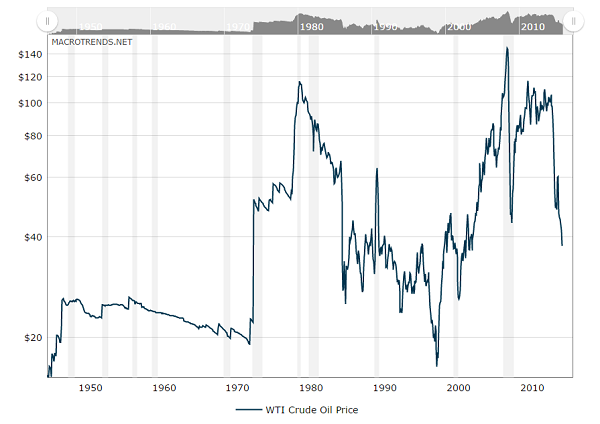
\includegraphics[width=0.30\textwidth]{img-000.png} &
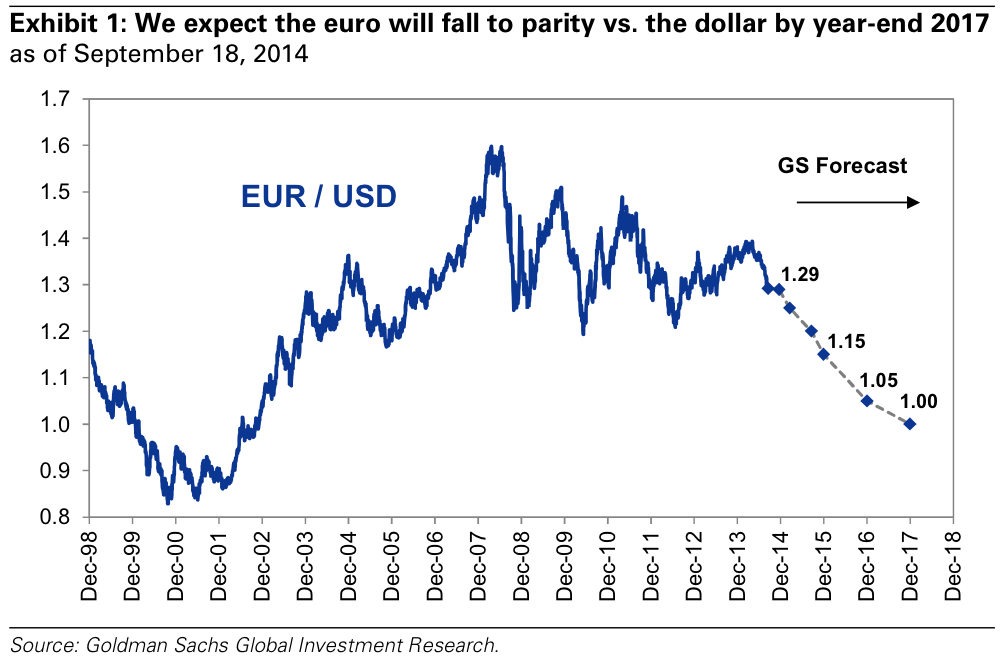
\includegraphics[width=0.30\textwidth]{img-005.png} &
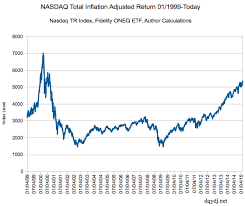
\includegraphics[width=0.30\textwidth]{img-010.png} \\
{\scriptsize Commodity (WTI)} &
{\scriptsize FX (EUR/USD)} &
{\scriptsize Equity index (NASDAQ)} \\
\end{tabular}
\end{center}
\end{frame}

% -----------------------------------------------------
\begin{frame}{From price to fluctuations: returns as ``increments''}
\begin{itemize}
  \item Prices are often \textbf{non-stationary} (trend + growth).\pause
  \item Work with \textbf{increments} or \textbf{log-returns}:
  \[
    R_{t,t+\Delta t}=\log S_{t+\Delta t}-\log S_t.\pause
  \]
  \item Empirically, for short horizons, returns look:
  \begin{itemize}
    \item centered (small mean),\pause
    \item noisy (variance proportional to horizon),\pause
    \item weakly dependent (not i.i.d., but a good starting point).\pause
  \end{itemize}
\end{itemize}

\medskip
\begin{exampleblock}{Mental model}
Think of ``new information'' arriving continuously $\Rightarrow$ small unpredictable shocks add up.
\end{exampleblock}
\end{frame}


% =====================================================
\section{Brownian motion as a limit of a random walk}

% -----------------------------------------------------
\begin{frame}{Step 1: the simple random walk}
Let $(\varepsilon_k)_{k\ge1}$ be i.i.d.\ with
\[
\mathbb{P}(\varepsilon_k=+1)=\mathbb{P}(\varepsilon_k=-1)=\tfrac12.\pause
\]
Define the random walk
\[
S_n=\sum_{k=1}^n \varepsilon_k,\qquad S_0=0.\pause
\]

\begin{itemize}
  \item $S_n$ is discrete in time and space.\pause
  \item Increments are independent and stationary.\pause
  \item $\mathbb{E}[S_n]=0,\quad \mathrm{Var}(S_n)=n$.
\end{itemize}
\end{frame}

% -----------------------------------------------------
\begin{frame}{Step 2: rescale time and space}
To get a \textbf{non-degenerate} limit as time becomes continuous:
\[
W^{(n)}(t)
=
\frac{1}{\sqrt{n}}\,S_{\lfloor nt\rfloor},
\qquad t\in[0,1].\pause
\]

\begin{exampleblock}{Why the factor $1/\sqrt{n}$?}
Because $\mathrm{Var}(S_{\lfloor nt\rfloor})\approx nt$.
Dividing by $\sqrt{n}$ yields $\mathrm{Var}(W^{(n)}(t))\approx t$.
\end{exampleblock}
\end{frame}

% -----------------------------------------------------
\begin{frame}{Picture: discrete walk vs.\ scaled walk}
\begin{center}
\begin{tikzpicture}
\node[anchor=west] at (0,3.3) {\small \textbf{(A) Random walk $S_{\lfloor nt\rfloor}$ (discrete scale)}};
\node[anchor=west] at (0,-0.2) {\small \textbf{(B) Scaled walk $W^{(n)}(t)=S_{\lfloor nt\rfloor}/\sqrt{n}$ (diffusive scale)}};

\begin{axis}[
  at={(0,1.55)}, anchor=south west,
  width=12cm,height=3.5cm,
  xmin=0,xmax=1,
  axis lines=left,
  xlabel={$t$}, ylabel={$S$},
  ytick=\empty, xtick=\empty,
]
\addplot[thick, BootcampBlueDark]
coordinates {
(0.0000,0.0000)
(0.0125,1.0000)
(0.0250,0.0000)
(0.0375,1.0000)
(0.0500,0.0000)
(0.0625,1.0000)
(0.0750,2.0000)
(0.0875,3.0000)
(0.1000,4.0000)
(0.1125,3.0000)
(0.1250,4.0000)
(0.1375,3.0000)
(0.1500,4.0000)
(0.1625,3.0000)
(0.1750,4.0000)
(0.1875,3.0000)
(0.2000,2.0000)
(0.2125,1.0000)
(0.2250,0.0000)
(0.2375,1.0000)
(0.2500,0.0000)
(0.2625,-1.0000)
(0.2750,-2.0000)
(0.2875,-1.0000)
(0.3000,0.0000)
(0.3125,-1.0000)
(0.3250,-2.0000)
(0.3375,-1.0000)
(0.3500,0.0000)
(0.3625,-1.0000)
(0.3750,-2.0000)
(0.3875,-1.0000)
(0.4000,-2.0000)
(0.4125,-3.0000)
(0.4250,-2.0000)
(0.4375,-1.0000)
(0.4500,-2.0000)
(0.4625,-3.0000)
(0.4750,-2.0000)
(0.4875,-1.0000)
(0.5000,-2.0000)
(0.5125,-1.0000)
(0.5250,0.0000)
(0.5375,-1.0000)
(0.5500,-2.0000)
(0.5625,-3.0000)
(0.5750,-2.0000)
(0.5875,-3.0000)
(0.6000,-4.0000)
(0.6125,-5.0000)
(0.6250,-6.0000)
(0.6375,-5.0000)
(0.6500,-4.0000)
(0.6625,-3.0000)
(0.6750,-2.0000)
(0.6875,-3.0000)
(0.7000,-2.0000)
(0.7125,-3.0000)
(0.7250,-2.0000)
(0.7375,-3.0000)
(0.7500,-4.0000)
(0.7625,-5.0000)
(0.7750,-4.0000)
(0.7875,-3.0000)
(0.8000,-4.0000)
(0.8125,-5.0000)
(0.8250,-6.0000)
(0.8375,-5.0000)
(0.8500,-4.0000)
(0.8625,-5.0000)
(0.8750,-4.0000)
(0.8875,-3.0000)
(0.9000,-4.0000)
(0.9125,-3.0000)
(0.9250,-2.0000)
(0.9375,-1.0000)
(0.9500,-2.0000)
(0.9625,-1.0000)
(0.9750,-2.0000)
(0.9875,-1.0000)
(1.0000,-2.0000)
};
\end{axis}

\begin{axis}[
  at={(0,0)}, anchor=south west,
  width=12cm,height=3.5cm,
  xmin=0,xmax=1,
  axis lines=left,
  xlabel={$t$}, ylabel={$W^{(n)}$},
  ytick=\empty, xtick=\empty,
]
\addplot[thick, BootcampBlue]
coordinates {
(0.0000,0.0000)
(0.0125,0.1118)
(0.0250,0.0000)
(0.0375,0.1118)
(0.0500,0.0000)
(0.0625,0.1118)
(0.0750,0.2236)
(0.0875,0.3354)
(0.1000,0.4472)
(0.1125,0.3354)
(0.1250,0.4472)
(0.1375,0.3354)
(0.1500,0.4472)
(0.1625,0.3354)
(0.1750,0.4472)
(0.1875,0.3354)
(0.2000,0.2236)
(0.2125,0.1118)
(0.2250,0.0000)
(0.2375,0.1118)
(0.2500,0.0000)
(0.2625,-0.1118)
(0.2750,-0.2236)
(0.2875,-0.1118)
(0.3000,0.0000)
(0.3125,-0.1118)
(0.3250,-0.2236)
(0.3375,-0.1118)
(0.3500,0.0000)
(0.3625,-0.1118)
(0.3750,-0.2236)
(0.3875,-0.1118)
(0.4000,-0.2236)
(0.4125,-0.3354)
(0.4250,-0.2236)
(0.4375,-0.1118)
(0.4500,-0.2236)
(0.4625,-0.3354)
(0.4750,-0.2236)
(0.4875,-0.1118)
(0.5000,-0.2236)
(0.5125,-0.1118)
(0.5250,0.0000)
(0.5375,-0.1118)
(0.5500,-0.2236)
(0.5625,-0.3354)
(0.5750,-0.2236)
(0.5875,-0.3354)
(0.6000,-0.4472)
(0.6125,-0.5590)
(0.6250,-0.6708)
(0.6375,-0.5590)
(0.6500,-0.4472)
(0.6625,-0.3354)
(0.6750,-0.2236)
(0.6875,-0.3354)
(0.7000,-0.2236)
(0.7125,-0.3354)
(0.7250,-0.2236)
(0.7375,-0.3354)
(0.7500,-0.4472)
(0.7625,-0.5590)
(0.7750,-0.4472)
(0.7875,-0.3354)
(0.8000,-0.4472)
(0.8125,-0.5590)
(0.8250,-0.6708)
(0.8375,-0.5590)
(0.8500,-0.4472)
(0.8625,-0.5590)
(0.8750,-0.4472)
(0.8875,-0.3354)
(0.9000,-0.4472)
(0.9125,-0.3354)
(0.9250,-0.2236)
(0.9375,-0.1118)
(0.9500,-0.2236)
(0.9625,-0.1118)
(0.9750,-0.2236)
(0.9875,-0.1118)
(1.0000,-0.2236)
};
\end{axis}
\end{tikzpicture}
\end{center}

\vspace{-1mm}
\begin{itemize}
  \item After scaling, the path ``stays of order 1'' and starts resembling a continuous object.
\end{itemize}
\end{frame}

% -----------------------------------------------------
\begin{frame}{CLT explains Gaussian increments}
For $0\le s<t\le 1$,
\[
W^{(n)}(t)-W^{(n)}(s)
=
\frac{1}{\sqrt{n}}
\sum_{k=\lfloor ns\rfloor+1}^{\lfloor nt\rfloor} \varepsilon_k.\pause
\]

\begin{itemize}
  \item Sum of $\approx n(t-s)$ i.i.d.\ centered variables.\pause
  \item By CLT, increments are approximately Gaussian:
  \[
  W^{(n)}(t)-W^{(n)}(s)\approx \mathcal{N}(0,\,t-s).\pause
  \]
\end{itemize}

\begin{exampleblock}{Takeaway}
Brownian motion is the continuous-time object whose increments behave like CLT limits.
\end{exampleblock}
\end{frame}

% -----------------------------------------------------
\begin{frame}{Invariance principle (informal statement)}
\begin{definitionblock}{Donsker's invariance principle (informal)}
As $n\to\infty$, the process $W^{(n)}(\cdot)$ converges in distribution (as a random function) to
a process $W(\cdot)$ called \textbf{Brownian motion}.\pause
\end{definitionblock}

\begin{itemize}
  \item Same scaling limit for many i.i.d.\ increments (not only $\pm 1$).\pause
  \item Robust explanation for the ubiquity of Brownian motion.
\end{itemize}
\end{frame}

% =====================================================
\section{Continuous-time processes and filtrations}

% -----------------------------------------------------
\begin{frame}{Stochastic processes in continuous time}
A \textbf{stochastic process} is a family $(X_t)_{t\ge0}$ of random variables.\pause

\medskip
\begin{itemize}
  \item Discrete time: $t\in\{0,1,2,\dots\}$.\pause
  \item Continuous time: $t\in[0,\infty)$.\pause
\end{itemize}

\medskip
\begin{exampleblock}{Examples}
\begin{itemize}
  \item Price process $S_t$, short rate $r_t$, volatility $\sigma_t$.\pause
  \item Queue length, population size, temperature signal.
\end{itemize}
\end{exampleblock}
\end{frame}

% -----------------------------------------------------
\begin{frame}{Filtration = flow of information}
\begin{definitionblock}{Filtration}
A filtration $(\mathcal{F}_t)_{t\ge0}$ is an increasing family of $\sigma$-algebras:
\[
\mathcal{F}_s\subseteq \mathcal{F}_t \quad \text{for } s\le t.\pause
\]
\end{definitionblock}

\begin{itemize}
  \item $\mathcal{F}_t$ represents \textbf{everything you know up to time $t$}.\pause
  \item ``More time $\Rightarrow$ more information''.\pause
\end{itemize}

\medskip
\begin{center}
\begin{tikzpicture}[>=Stealth]
\draw[->,thick] (0,0) -- (10,0) node[right] {$t$};
\foreach \x/\lab in {0/0,2/1,4/2,6/3,8/4} {
  \draw (\x,0.12) -- (\x,-0.12);
  \node[below] at (\x,-0.12) {\scriptsize $\lab$};
}
\node[above] at (1,0.25) {\scriptsize $\mathcal{F}_0$};
\node[above] at (3,0.25) {\scriptsize $\mathcal{F}_1$};
\node[above] at (5,0.25) {\scriptsize $\mathcal{F}_2$};
\node[above] at (7,0.25) {\scriptsize $\mathcal{F}_3$};
\node[above] at (9,0.25) {\scriptsize $\mathcal{F}_4$};

\draw[decorate,decoration={brace,amplitude=5pt},thick,AccentGold]
  (0,-0.8) -- (10,-0.8);
\node at (5,-1.2) {\small information grows with time};
\end{tikzpicture}
\end{center}
\end{frame}

% -----------------------------------------------------
\begin{frame}{Adaptedness and stopping times (very practical)}
\begin{definitionblock}{Adapted process}
$(X_t)$ is \textbf{adapted} to $(\mathcal{F}_t)$ if $X_t$ is $\mathcal{F}_t$-measurable for each $t$.\pause
\end{definitionblock}

\medskip
\begin{definitionblock}{Stopping time}
A random time $\tau$ is a stopping time if $\{\tau\le t\}\in\mathcal{F}_t$ for all $t$.\pause
\end{definitionblock}

\medskip
\begin{itemize}
  \item ``At time $t$, you can decide whether the event has happened.''\pause
  \item Examples: first time a stock hits a barrier; first time a drawdown exceeds $10\%$.
\end{itemize}
\end{frame}

% =====================================================
\section{Brownian motion: definition, properties, and roughness}

% -----------------------------------------------------
\begin{frame}{Definition of Brownian motion}
\begin{definitionblock}{Standard Brownian motion}
A process $(W_t)_{t\ge0}$ is a \textbf{Brownian motion} if:\pause
\begin{enumerate}
  \item $W_0=0$ a.s.\pause
  \item Independent increments: $W_t-W_s$ independent of $\mathcal{F}_s$ for $s<t$.\pause
  \item Gaussian increments: $W_t-W_s\sim\mathcal{N}(0,t-s)$.\pause
  \item Almost surely continuous paths.\pause
\end{enumerate}
\end{definitionblock}

\medskip
\begin{itemize}
  \item Think: ``continuous limit of many tiny independent shocks.''
\end{itemize}
\end{frame}

% -----------------------------------------------------
\begin{frame}{A Gaussian process viewpoint (one formula to remember)}
\begin{itemize}
  \item Brownian motion is a centered Gaussian process.\pause
  \item Its covariance fully specifies the joint laws:
  \[
  \mathbb{E}[W_s W_t]=\min(s,t).\pause
  \]
\end{itemize}

\medskip
\begin{exampleblock}{Consequences}
\begin{itemize}
  \item $\mathbb{E}[W_t]=0$, $\mathrm{Var}(W_t)=t$.\pause
  \item For any $(t_1,\dots,t_k)$, $(W_{t_1},\dots,W_{t_k})$ is multivariate normal.\pause
\end{itemize}
\end{exampleblock}
\end{frame}

% -----------------------------------------------------
\begin{frame}{Martingale and Markov properties}
\begin{itemize}
  \item \textbf{Martingale:} $\mathbb{E}[W_t\mid\mathcal{F}_s]=W_s$ for $s\le t$.\pause
  \item \textbf{Markov:} conditional on $W_s$, the future depends only on $W_s$.\pause
\end{itemize}

\medskip
\begin{exampleblock}{Finance intuition}
If $S_t=S_0\exp\big((r-\tfrac12\sigma^2)t+\sigma W_t\big)$, then (under risk-neutral pricing)
discounted $e^{-rt}S_t$ is a martingale.\pause
\end{exampleblock}
\end{frame}

% -----------------------------------------------------
\begin{frame}{Self-similarity (scaling) and why it matters}
For any $c>0$,
\[
\big(W_{ct}\big)_{t\ge0}
\ \overset{d}{=}\
\big(\sqrt{c}\,W_t\big)_{t\ge0}.\pause
\]

\begin{itemize}
  \item Zoom in time by factor $c$ $\Rightarrow$ vertical scale grows by $\sqrt{c}$.\pause
  \item Explains why Brownian paths look ``similar'' at different magnifications.
\end{itemize}
\end{frame}

% -----------------------------------------------------
\begin{frame}{Brownian motion is \emph{not} differentiable (intuition)}
If $W$ were differentiable, we would expect
\[
\frac{W_{t+\Delta t}-W_t}{\Delta t}
\quad \text{to stay bounded as }\Delta t\to0.\pause
\]

But Brownian increments satisfy
\[
W_{t+\Delta t}-W_t \sim \mathcal{N}(0,\Delta t)
\quad\Rightarrow\quad
|W_{t+\Delta t}-W_t|\ \text{is typically of size }\sqrt{\Delta t}.\pause
\]

So
\[
\left|\frac{W_{t+\Delta t}-W_t}{\Delta t}\right|
\approx
\frac{\sqrt{\Delta t}}{\Delta t}
=
\frac{1}{\sqrt{\Delta t}}
\ \longrightarrow\ \infty.\pause
\]

\begin{exampleblock}{Key message}
Brownian motion has infinite ``instantaneous slope'' almost everywhere.\pause
\end{exampleblock}
\end{frame}

% =====================================================
\section{Quadratic variation and the need for a new integral}

% -----------------------------------------------------
\begin{frame}{Quadratic variation: a fingerprint of Brownian motion}
Take a partition $0=t_0<t_1<\cdots<t_n=t$ and define
\[
QV_t^{(\pi)}=\sum_{k=0}^{n-1}\big(W_{t_{k+1}}-W_{t_k}\big)^2.\pause
\]

\begin{definitionblock}{Quadratic variation}
The quadratic variation of $W$ on $[0,t]$ is the limit (in probability)
\[
[W]_t=\lim_{|\pi|\to0} QV_t^{(\pi)}.\pause
\]
\end{definitionblock}

\medskip
\begin{exampleblock}{Two contrasts}
\begin{itemize}
  \item Smooth function $f(t)$: $\sum (f(t_{k+1})-f(t_k))^2\to 0$.\pause
  \item Brownian motion: the limit is \textbf{non-zero}.
\end{itemize}
\end{exampleblock}
\end{frame}

% -----------------------------------------------------
\begin{frame}{Computation: for Brownian motion, $[W]_t=t$}
Heuristic with equal mesh $\Delta t=t/n$:
\[
\mathbb{E}\!\left[\sum_{k=0}^{n-1}(W_{t_{k+1}}-W_{t_k})^2\right]
=
\sum_{k=0}^{n-1}\mathbb{E}\big[(W_{t_{k+1}}-W_{t_k})^2\big]
=
n\cdot \Delta t = t.
\]

\medskip
One can show that the variance of the sum goes to $0$ as $n\to\infty$,
so the sum converges in probability to $t$:
\[
[W]_t=t.\pause
\]

\begin{exampleblock}{Why this is huge}
Quadratic variation replaces the missing derivative in calculus with Brownian motion.
\end{exampleblock}
\end{frame}

% -----------------------------------------------------
\begin{frame}{Why we need a new integral}
For smooth $x(t)$, Riemann sums
\[
\sum f(t_k)\big(x(t_{k+1})-x(t_k)\big)\pause
\]
converge to $\int f\,dx$.

\medskip
For Brownian motion:
\begin{itemize}
  \item increments are random and of size $\sqrt{\Delta t}$,\pause
  \item quadratic variation is non-zero,\pause
  \item naive ``pathwise'' limits are delicate.
\end{itemize}

\begin{definitionblock}{It\^o integral (idea)}
Define $\int_0^t H_s\,dW_s$ as an $L^2$-limit of sums
\[
\sum_{k} H_{t_k}\big(W_{t_{k+1}}-W_{t_k}\big)
\quad \text{with } H_{t_k}\ \text{known at time } t_k.\pause
\]
\end{definitionblock}
\end{frame}

% -----------------------------------------------------
\begin{frame}{Stochastic Integral as the Limit of Discrete Rebalancing (Bachelier)}
\textbf{Start in discrete time: trading on a grid.}
Fix \(0=t_0<t_1<\cdots<t_n=T\). Let $(S_t)$ be the price of a stock.
A trader chooses at each date \(t_k\) the number of shares \(\Delta_{t_k}\),
based on information available at time \(t_k\) (i.e.\ \(\Delta_{t_k}\) is \(\mathcal{F}_{t_k}\)-measurable).

\medskip
\textbf{Self-financing portfolio.}
Assume a bank account with \(r=0\) ($0$ interest rates, to keep formulas clean).\pause
If \(V_{t_k}\) is the portfolio value just after rebalancing at \(t_k\), then during \([t_k,t_{k+1}]\)
the number of shares is constant, so the gain is:
\[
V_{t_{k+1}}-V_{t_k}=\Delta_{t_k}\big(S_{t_{k+1}}-S_{t_k}\big).\pause
\]

\medskip
Summing increments,
\[
V_T
=
V_0+\sum_{k=0}^{n-1}\Delta_{t_k}\big(S_{t_{k+1}}-S_{t_k}\big).\pause
\]

\begin{definitionblock}{Discrete stochastic integral (left-point rule)}
\[
\sum_{k=0}^{n-1}\Delta_{t_k}\big(S_{t_{k+1}}-S_{t_k}\big)
\quad \text{with }\Delta_{t_k}\text{ known at time }t_k.\pause
\]
\end{definitionblock}

\medskip
\textbf{Interpretation:} ``Choose \(\Delta\) now, earn \(\Delta\times\) next price move.''
\end{frame}

% -----------------------------------------------------
\begin{frame}{Why Take a Limit? From Discrete Gains to $\int \Delta\,dS$}
\textbf{If we rebalance more and more often:}
take partitions with mesh \(\max_k (t_{k+1}-t_k)\to 0\).

\medskip
We would like the discrete gain
\[
\sum_{k=0}^{n-1}\Delta_{t_k}\big(S_{t_{k+1}}-S_{t_k}\big)
\]
to converge to a well-defined continuous-time object.

\medskip
\textbf{But with Brownian-type prices:}
\begin{itemize}
  \item increments are random of size \(\sqrt{\Delta t}\),\pause
  \item naive pathwise limits can fail / depend on the rule (left vs midpoint),\pause
  \item we need a definition that matches the information flow: \(\Delta_{t_k}\) decided \emph{before} seeing \(S_{t_{k+1}}\).\pause
\end{itemize}

\begin{definitionblock}{Goal}
Define a continuous-time gain process \(G_t\) such that
\[
G_T \approx \sum_{k}\Delta_{t_k}\big(S_{t_{k+1}}-S_{t_k}\big),
\qquad
\text{when the grid is fine.}
\]
\end{definitionblock}

\medskip
\textbf{This will be written } \(G_T=\int_0^T \Delta_t\,dS_t\).
\end{frame}

% -----------------------------------------------------
\begin{frame}{Bachelier Model and the Continuous-Time Limit}
\textbf{Bachelier model (additive Brownian motion).}
Assume
\[
S_t = S_0 + \sigma W_t,
\]

\medskip
Plugging into the discrete gain:
\[
\sum_{k=0}^{n-1}\Delta_{t_k}\big(S_{t_{k+1}}-S_{t_k}\big)
=
\sigma\sum_{k=0}^{n-1}\Delta_{t_k}\big(W_{t_{k+1}}-W_{t_k}\big).
\]

\medskip
\begin{definitionblock}{It\^o integral = limit of discrete gains}
We \emph{define} the stochastic integral by the limit (in \(L^2\), typically):
\[
\int_0^T \Delta_t\,dW_t
\ :=\
\lim_{\|\pi\|\to 0}\ \sum_{k}\Delta_{t_k}\big(W_{t_{k+1}}-W_{t_k}\big),
\]
with \(\Delta_{t_k}\) measurable w.r.t.\ \(\mathcal{F}_{t_k}\).\pause
\end{definitionblock}

\medskip
Therefore, the continuous-time trading gain becomes
\[
V_T = V_0 + \int_0^T \Delta_t\,dS_t
=
V_0 + \sigma\int_0^T \Delta_t\,dW_t.\pause
\]

\medskip
\textbf{Key message:}
\[
\text{stochastic integrals are the mathematical object behind ``rebalance \& hedge''.}
\]
\end{frame}

% -----------------------------------------------------
\begin{frame}{One key property: It\^o isometry (intuition)}
For a nice adapted process $H$,
\[
\mathbb{E}\!\left[\left(\int_0^t H_s\,dW_s\right)^2\right]
=
\mathbb{E}\!\left[\int_0^t H_s^2\,ds\right].\pause
\]

\begin{itemize}
  \item The ``variance'' of the stochastic integral is controlled by $\int H^2$.\pause
  \item This is the workhorse for existence and computations.\pause
\end{itemize}

\begin{exampleblock}{Finance hint}
If $H_s$ is your trading strategy (delta), then $\int H\,dS$ is the cumulative gain from trading.
\end{exampleblock}
\end{frame}

% =====================================================
\section{Semimartingales: extending calculus beyond differentiability}

% -----------------------------------------------------
\begin{frame}{From differentiable functions to semimartingales}
A differentiable path satisfies:
\[
dx_t = \dot x_t\,dt,
\qquad [x]_t=0.\pause
\]

\medskip
A \textbf{semimartingale} decomposes as
\[
X_t = X_0 + A_t + M_t,\pause
\]
where
\begin{itemize}
  \item $A_t$ has finite variation (``drift-like''),
  \item $M_t$ is a local martingale (``noise-like'').
\end{itemize}

\begin{exampleblock}{Prototype: It\^o process}
\[
dX_t = b_t\,dt + \sigma_t\,dW_t.\pause
\]
\end{exampleblock}
\end{frame}

% -----------------------------------------------------
\begin{frame}{It\^o formula (chain rule with a correction term)}
If $X_t$ is an It\^o process and $f\in C^2$, then
\[
df(X_t)
=
f'(X_t)\,dX_t
+\frac12 f''(X_t)\,d[X]_t.\pause
\]

For $dX_t=b_t\,dt+\sigma_t\,dW_t$ and $[X]_t=\int_0^t \sigma_s^2\,ds$:
\[
df(X_t)=f'(X_t)b_t\,dt + f'(X_t)\sigma_t\,dW_t + \frac12 f''(X_t)\sigma_t^2\,dt.\pause
\]

\begin{exampleblock}{Why the extra term?}
Because Brownian motion has quadratic variation: $[W]_t=t$.
\end{exampleblock}
\end{frame}

% -----------------------------------------------------
\begin{frame}{Concrete finance example: geometric Brownian motion}
Assume a stock follows
\[
dS_t=\mu S_t\,dt + \sigma S_t\,dW_t.\pause
\]

Apply It\^o to $f(s)=\log s$:
\[
d(\log S_t)=\left(\mu-\tfrac12\sigma^2\right)\!dt + \sigma\,dW_t.
\]

\begin{itemize}
  \item Drift of log-price is reduced by $\tfrac12\sigma^2$ (the It\^o correction).
  \item This is the backbone of Black--Scholes modeling.
\end{itemize}
\end{frame}

% -----------------------------------------------------
\begin{frame}{Model 1: Risk-neutral GBM (Black--Scholes world)}
\textbf{Under the pricing measure $\mathbb{Q}$}, the stock is modeled as
\[
dS_t = r S_t\,dt + \sigma S_t\,dW_t^{\mathbb{Q}}.\pause
\]
Then the \textbf{discounted price} is a martingale:
\[
\tilde S_t := e^{-rt}S_t
\quad\Rightarrow\quad
d\tilde S_t = \sigma \tilde S_t\, dW_t^{\mathbb{Q}}.
\]

\medskip
\textbf{Closed form (solution of the SDE):}
\[
S_t = S_0\exp\!\Big((r-\tfrac12\sigma^2)t+\sigma W_t^{\mathbb{Q}}\Big).\pause
\]

\medskip
\begin{itemize}
  \item Gives lognormal returns.
  \item Pricing reduces to computing $\mathbb{Q}$-expectations (Black--Scholes).
\end{itemize}
\end{frame}

% -----------------------------------------------------
\begin{frame}{Model 2: Brownian motion with drift for log-returns (short horizon)}
A simple short-horizon model for \textbf{log-returns}:
\[
X_t := \log\!\Big(\frac{S_t}{S_0}\Big)
= \alpha t + \sigma W_t.
\]

\medskip
\textbf{Implications:}
\begin{itemize}
  \item $X_t \sim \mathcal{N}(\alpha t,\sigma^2 t)$.
  \item Over $\Delta t$: \quad $X_{t+\Delta t}-X_t \sim \mathcal{N}(\alpha\Delta t,\sigma^2\Delta t)$.
\end{itemize}

\medskip
\textbf{Calibration intuition:}
\begin{itemize}
  \item $\sigma$ from realized volatility (scales like $\sqrt{\Delta t}$).
  \item $\alpha$ is small and noisy; pricing often focuses on $\sigma$.
\end{itemize}
\end{frame}

% -----------------------------------------------------
\begin{frame}{Model 3: Vasicek short-rate model (Gaussian rates)}
Model the short rate $r_t$ by mean-reversion:
\[
dr_t = a(b-r_t)\,dt + \sigma\, dW_t.
\]

\medskip
\textbf{Why finance likes it:}
\begin{itemize}
  \item Rates revert toward long-run level $b$ at speed $a$.
  \item Gaussian and analytically tractable $\Rightarrow$ bond prices in closed form.
\end{itemize}

\medskip
\textbf{Key takeaway:}
\[
r_t \mid r_s \ \text{is Gaussian, and }\ \mathbb{E}[r_t\mid r_s]=b+(r_s-b)e^{-a(t-s)}.
\]

\medskip
\textbf{Limitation (important!):} can produce negative rates.
\end{frame}

% -----------------------------------------------------
\begin{frame}{Model 4: CIR short-rate model (positive rates)}
A popular alternative that \textbf{keeps rates nonnegative}:
\[
dr_t = a(b-r_t)\,dt + \sigma\sqrt{r_t}\, dW_t.
\]

\medskip
\textbf{Interpretation:}
\begin{itemize}
  \item Mean reversion as before.
  \item Volatility increases with $\sqrt{r_t}$: when rates are high, uncertainty is higher.
\end{itemize}

\medskip
\textbf{Why it matters in pricing:}
\begin{itemize}
  \item More realistic term-structure dynamics.
  \item Still tractable: many bond prices have closed forms (affine model).
\end{itemize}

\medskip
\textbf{Rule of thumb:} $\sqrt{r_t}$ noise prevents negative rates (under a condition).
\end{frame}

% -----------------------------------------------------
\begin{frame}{Model 5: Stochastic volatility (Heston-style intuition)}
Empirically, volatility is not constant. A simple two-factor idea:
\[
\begin{cases}
dS_t = r S_t\,dt + \sqrt{v_t}\,S_t\, dW_t^{(1)},\\
dv_t = \kappa(\theta-v_t)\,dt + \xi\sqrt{v_t}\, dW_t^{(2)},\\
d\langle W^{(1)},W^{(2)}\rangle_t = \rho\,dt.
\end{cases}
\]

\medskip
\textbf{What each parameter does:}
\begin{itemize}
  \item $\kappa,\theta$: mean reversion of variance (vol ``clusters'').
  \item $\rho<0$: leverage effect (down moves $\Rightarrow$ vol up).
  \item $\xi$: vol-of-vol (smile/skew strength).
\end{itemize}

\medskip
\textbf{Use case:} explains implied-volatility smiles better than constant-$\sigma$.
\end{frame}

% -----------------------------------------------------
\begin{frame}{Model 6: Jump-diffusion for crash risk (Merton intuition)}
To capture sudden moves, add jumps:
\[
\frac{dS_t}{S_{t^-}} = r\,dt + \sigma\, dW_t + (J-1)\, dN_t,
\]
where $N_t$ is a Poisson process (intensity $\lambda$) and $J$ is the jump multiplier.

\medskip
\textbf{Interpretation:}
\begin{itemize}
  \item Continuous ``normal'' variation via Brownian motion.
  \item Rare events via jumps (earnings surprises, news shocks, crashes).
\end{itemize}

\medskip
\textbf{Practical effect:}
\begin{itemize}
  \item Generates heavier tails in returns.
  \item Produces steeper implied-vol smiles/skews (especially short maturities).
\end{itemize}
\end{frame}

% -----------------------------------------------------
\begin{frame}{Wrap-up: what to remember}
\begin{itemize}
  \item Brownian motion is the continuous-time limit of many random walks (diffusive scaling).
  \item Filtration is a \textbf{model of information} available over time.
  \item Brownian paths are continuous but \textbf{not differentiable}.
  \item Quadratic variation $[W]_t=t$ is the key new feature $\Rightarrow$ It\^o integral + It\^o formula.
  \item Semimartingales unify ``drift + noise'' and make stochastic calculus work.
\end{itemize}

\medskip
\centering
\textcolor{BootcampBlueDark}{Next: SDEs, Black--Scholes, and optional stopping / martingale methods.}
\end{frame}

\end{document}
